% fig3_spindle.tex: prescribed symmetric body inside the ambient color model
% Standalone source for the figure PDF of the same name.
% Build:  pdflatex fig3_spindle.tex
% Drawing from the frozen July manuscript, jmp/Magenta_Gap_JMP.tex, lines 615-682, with one label changed:
% "chimerical colors" now reads "outside the modeled ordinary image".
% Rebuilt as a standalone vector drawing so that the PDF contains only the figure.
% The border pads the drawing to 260 x 155 pt, the size of the file it replaces,
% so the figure keeps its reviewed scale in the manuscript.
\documentclass[tikz,border={15.08pt 10.88pt}]{standalone}
\usepackage[T1]{fontenc}
\usepackage{lmodern}
\usepackage{amsmath,amssymb}
\usepackage{xcolor}
\usetikzlibrary{arrows.meta,positioning,calc,decorations.pathreplacing}
\begin{document}
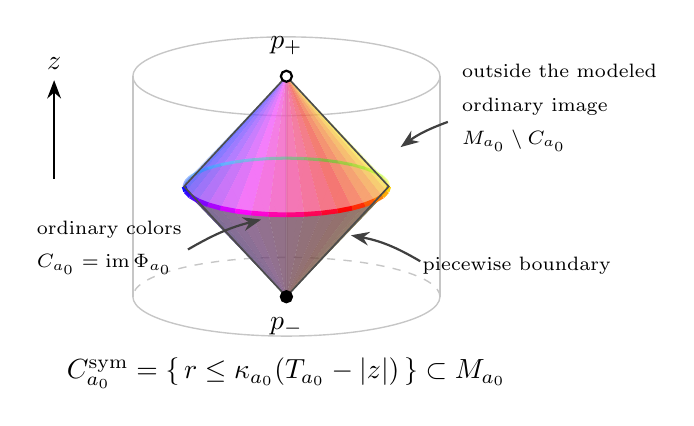
\begin{tikzpicture}[>=Stealth, line width=0.8pt]

  \draw[gray!45,dashed,line width=0.5pt] (1.95,-1.4) arc[start angle=0,end angle=180,x radius=1.95,y radius=0.5];
  \draw[gray!45,line width=0.5pt]         (1.95,-1.4) arc[start angle=0,end angle=-180,x radius=1.95,y radius=0.5];
  \draw[gray!45,line width=0.5pt] (-1.95,-1.4)--(-1.95,1.4);
  \draw[gray!45,line width=0.5pt] ( 1.95,-1.4)--( 1.95,1.4);
  \draw[gray!45,line width=0.5pt] (0,1.4) ellipse[x radius=1.95,y radius=0.5];

  \foreach \i in {0,...,17}{
    \pgfmathsetmacro{\pa}{\i*10}\pgfmathsetmacro{\pb}{(\i+1)*10}
    \pgfmathsetmacro{\hueval}{mod(\i/36+0.16667,1)}
    \definecolor{hh}{hsb}{\hueval,1,1}
    \pgfmathsetmacro{\xa}{1.3*cos(\pa)}\pgfmathsetmacro{\ya}{0.36*sin(\pa)}
    \pgfmathsetmacro{\xb}{1.3*cos(\pb)}\pgfmathsetmacro{\yb}{0.36*sin(\pb)}
    \fill[hh!52!black,fill opacity=0.18] (\xa,\ya)--(\xb,\yb)--(0,-1.4)--cycle;
    \fill[hh!78!white,fill opacity=0.18] (\xa,\ya)--(\xb,\yb)--(0, 1.4)--cycle;
  }

  \draw[gray!60,line width=1pt,opacity=0.55] (0,-1.32)--(0,1.32);

  \foreach \i in {18,...,35}{
    \pgfmathsetmacro{\pa}{\i*10}\pgfmathsetmacro{\pb}{(\i+1)*10}
    \pgfmathsetmacro{\hueval}{mod(\i/36+0.16667,1)}
    \definecolor{hh}{hsb}{\hueval,1,1}
    \pgfmathsetmacro{\xa}{1.3*cos(\pa)}\pgfmathsetmacro{\ya}{0.36*sin(\pa)}
    \pgfmathsetmacro{\xb}{1.3*cos(\pb)}\pgfmathsetmacro{\yb}{0.36*sin(\pb)}
    \fill[hh!45!black,fill opacity=0.70] (\xa,\ya)--(\xb,\yb)--(0,-1.4)--cycle;
    \fill[hh!72!white,fill opacity=0.70] (\xa,\ya)--(\xb,\yb)--(0, 1.4)--cycle;
  }

  \foreach \i in {0,...,17}{
    \pgfmathsetmacro{\pa}{\i*10}\pgfmathsetmacro{\pb}{(\i+1)*10}
    \pgfmathsetmacro{\hueval}{mod(\i/36+0.16667,1)}\definecolor{hh}{hsb}{\hueval,1,1}
    \draw[hh,line width=1.1pt,opacity=0.40]
      ({1.3*cos(\pa)},{0.36*sin(\pa)})--({1.3*cos(\pb)},{0.36*sin(\pb)});
  }
  \foreach \i in {18,...,35}{
    \pgfmathsetmacro{\pa}{\i*10}\pgfmathsetmacro{\pb}{(\i+1)*10}
    \pgfmathsetmacro{\hueval}{mod(\i/36+0.16667,1)}\definecolor{hh}{hsb}{\hueval,1,1}
    \draw[hh,line width=1.7pt,opacity=0.95]
      ({1.3*cos(\pa)},{0.36*sin(\pa)})--({1.3*cos(\pb)},{0.36*sin(\pb)});
  }

  \draw[black!70,line width=0.6pt]
    (0,-1.4)--(1.3,0)--(0,1.4)--(-1.3,0)--cycle;

  \filldraw[draw=black,fill=white] (0, 1.4) circle (2pt);
  \filldraw[draw=black,fill=black] (0,-1.4) circle (2pt);
  \node[above=1pt] at (0,1.5){$p_+$};
  \node[below=1pt] at (0,-1.5){$p_-$};

  \draw[->] (-2.95,0.1)--(-2.95,1.35);
  \node[above] at (-2.95,1.35){$z$};

  \node[anchor=west,align=left] at (-3.3,-0.78)
    {\scriptsize ordinary colors\\ \scriptsize $C_{a_0}=\operatorname{im}\Phi_{a_0}$};
  \draw[->,gray!50!black] (-1.25,-0.8) to[bend left=8] (-0.32,-0.42);
  \node[anchor=west,align=left] at (2.1,1.0)
    {\scriptsize outside the modeled\\ \scriptsize ordinary image\\ \scriptsize $M_{a_0}\setminus C_{a_0}$};
  \draw[->,gray!50!black] (2.05,0.82) to[bend right=8] (1.45,0.5);
  \node[anchor=west] at (1.6,-1.0){\scriptsize piecewise boundary};
  \draw[->,gray!50!black] (1.7,-0.95) to[bend right=10] (0.82,-0.62);

  \node[anchor=north] at (0,-2.05)
    {$C_{a_0}^{\mathrm{sym}}=\{\,r\le\kappa_{a_0}(T_{a_0}-|z|)\,\}
    \subset M_{a_0}$};

\end{tikzpicture}
\end{document}
